\setcounter{section}{8}

\section{Синтаксичний аналіз без повернення назад}

\subsubsection{Проблеми загальних граматик}

При виведенні слова $\omega$ в $G$ на кожному кроці безпосереднього виведення, коли ми беремо до уваги виділений нами нетермінал (в залежності від стратегії виведення), виникає питання, яку альтернативу для $A_i$ використати. З точки зору практики, нас цікавить така стратегія виведення $\omega$ в граматиці $G$, коли кожний наступний крок безпосереднього виведення наближав би нас до мети. Ця стратегія дасть можливість виконати виведення $\omega$ в $G$ за час $O(n)$, де $n = |\omega|$. \medskip

Зрозуміло, що не маючи інформації про структуру $\omega$, досягнути вибраної нами мети в більшості випадків неможливо. Але ж тримати інформацію про все слово $\omega$ також недопустимо. З точки зору практики, отримати потрібний результат розумно при наявності локальної інформації, наприклад, $k$ поточних вхідних лексем програми ($k$ --- наперед фіксоване число) достатньо для організації виведення $\omega$ в $G$ за час $O(n)$. З точки зору синтаксичного аналізу слова $\omega$ мова ведеться про наступну ситуацію:
\begin{figure}[H]
	\centering
	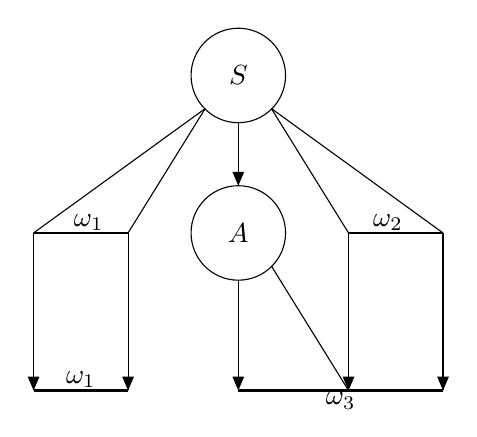
\begin{tikzpicture}[scale=0.2]
\tikzstyle{every node}+=[inner sep=0pt]
\draw [black] (0,0) circle (3);
\draw (0,0) node {$S$};

\draw [black] (-2.1, -2.1) -- (-7,-10);
\draw [black] (-2.1, -2.1) -- (-13,-10);
\draw [black, thick] (-7,-10) -- (-13, -10);
\draw (-9.5, -9.875) node [above] {$\omega_1$};

\draw [black] (0, -3) -- (0, -7);
\fill [black] (0, -7) -- (-.375, -6.125) -- (+.375, -6.125);
\draw [black] (0, -10) circle (3);
\draw (0, -10) node {$A$};

\draw [black] (+2.1, -2.1) -- (7,-10);
\draw [black] (+2.1, -2.1) -- (13,-10);
\draw [black, thick] (7,-10) -- (13, -10);
\draw (+9.5, -9.875) node [above] {$\omega_2$};

\draw [black] (-7, -10) -- (-7,-20);
\fill [black] (-7, -20) -- (-7.375, -19.125) -- (-6.625, -19.125);
\draw [black] (-13, -10) -- (-13,-20);
\fill [black] (-13, -20) -- (-13.375, -19.125) -- (-12.625, -19.125);
\draw [black, thick] (-7,-20) -- (-13, -20);
\draw (-10, -19.875) node [above] {$\omega_1$};

\draw [black] (0, -13) -- (0,-20);
\fill [black] (0, -20) -- (-.375, -19.125) -- (+.375, -19.125);
\draw [black] (+2.1, -12.1) -- (7,-20);
\draw [black] (+7, -10) -- (+7,-20);
\fill [black] (+7, -20) -- (+7.375, -19.125) -- (+6.625, -19.125);
\draw [black] (+13, -10) -- (+13,-20);
\fill [black] (+13, -20) -- (+13.375, -19.125) -- (+12.625, -19.125);
\draw [black, thick] (0,-20) -- (+13, -20);
\draw (+6.5, -20.125) node [below] {$\omega_3$};
\end{tikzpicture}

\end{figure}

Зафіксуємо стратегію виведення: далі будемо розглядати лише лівосторонню стратегію виведення $\omega$ в $G$. Тоді:
\begin{itemize}
	\item $S \Rightarrow^\star \omega_1 A \omega_2$ ($A$ --- перший зліва направо нетермінал);
	\item $\omega_1$ --- термінальна частина слова $\omega$, яку вже виведено (проаналізована частина слова);
	\item результат $\omega_3$, який потрібно ще вивести, виводиться зі слова $A \omega_2$;
	\item щоб зробити вірний крок виведення (без повернення назад) нам достатньо $k$ поточних  вхідних символів з непроаналізованої частини програми $\omega_3$.
\end{itemize}

Сформульовані умови забезпечує клас $LL(k)$-граматик.

\subsection{$LL(k)$-граматики}

КС-граматика $G = \left\langle N, \Sigma, P, S \right\rangle$ називається \textit{$LL(k)$-граматикою} для деякого фіксованого $k$, якщо для двох лівосторонніх виведень вигляду:
\begin{enumerate}
	\item $S \Rightarrow^\star \omega_1 A \omega_2 \Rightarrow \omega_1 \alpha \omega_2 \Rightarrow^\star \omega_1 x$;
	\item $S \Rightarrow^\star \omega_1 A \omega_2 \Rightarrow \omega_1 \beta \omega_2 \Rightarrow^\star \omega_1 y$;
\end{enumerate}
з $\text{First}_k (x) = \text{First}_k (y)$ випливає, що $\alpha = \beta$, де $A \mapsto \alpha \mid \beta$, а \[\text{First}_k(\alpha) = \left\{ \omega \mid \alpha \Rightarrow^\star \omega x,\vert\omega\vert = k \right\} \cup \left\{ \omega \mid \alpha \Rightarrow^\star \omega, \vert\omega\vert < k \right\}.\]

Неформально, граматика $G$ буде $LL(k)$-граматикою, якщо для слова \[\omega_1 A \omega_2 \in (N \cup \Sigma)^\star\] достатньо $k$ перших символів (за умови, що вони існують) решти непроаналізованого слова щоб визначити, що з $A \omega_2$ існує не більше однієї альтернативи виведення слова, що починається з $\omega$ та продовжується наступними $k$ термінальними символами. \medskip

Сформулюємо основні твердження стосовно класу $LL(k)$-граматик:
\begin{enumerate}
	\item Не існує алгоритма, який перевіряє належність КС-граматики класу $LL(k)$-граматик.
	\item Для кожного конкретного $k$ існує алгоритм, який перевіряє, чи є задана граматика $LL(k)$-граматикою.
	\item Якщо граматика є $LL(k)$-граматикою, то вона є $LL(k + p)$-граматикою, $(p \ge 1)$.
	\item Клас $LL(k)$-граматик --- це підклас КС-граматик, який не покриває його.
\end{enumerate}

Продемонструємо на \textbf{прикладі} справедливість останнього твердження. Розглянемо граматику $G$ з наступною схемою $P$: $S \mapsto S a \mid b$. \medskip

Мова, яку породжує наведена вище граматика $L(G) = \{ ba^i, i = 0, 1, \ldots \}$. Візьмемо виведення наступного слова $S \Rightarrow^{i+1} b a^i$. За визначенням $LL(k)$-граматики якщо покласти $A = S,$ $\omega_2 = a^i,$ $\alpha = S a,$ $\beta = b,$ то маємо отримати
\[\text{First}_k \left(S a a^i\right) \cap \text{First}_k \left(b a^i\right) = \varnothing.\]

Втім, для $i \ge k$ маємо:\[\text{First}_k \left(S a a^i\right) = \text{First}_k \left(b a^i\right) = \left\{b a^{k - 1}\right\}.\]

Таким чином, КС-граматика $G$ не може бути $LL(k)$-граматикою для жодного $k$. \medskip

Як наслідок, КС-граматика $G$, яка має ліворекурсивний нетермінал $A$ (нетермінал $A$ називається \textit{ліворекурсивним}, якщо в граматиці $G$ існує вивід виду $A \Rightarrow^\star A \omega$), не може бути $LL(k)$-граматикою. \medskip

З практичної точки зору в більшості випадків ми будемо користуватися $LL(1)$-граматиками. У класі $LL(1)$-граматик існує один цікавий підклас --- це розподілені $LL(1)$-граматики. \medskip

$LL(1)$-граматика називаються \textit{розподіленою}, якщо вона задовольняє наступним умовам:
\begin{itemize}
	\item у схемі $P$ граматики відсутні $\varepsilon$-правила (правила вигляду $A \mapsto \varepsilon$);
	\item для нетермінала $A$ праві частини $A$-правила починаються різними терміналами.
\end{itemize}

\subsubsection{$\text{First}_k$}

Зауважимо, що $\text{First}_k (\omega_1 \omega_2) = \text{First}_k (\omega_1) \oplus_k \text{First}_k (\omega_2)$, де $\oplus_k$ --- бінарна операція над словарними множинами (мовами) визначена наступним чином:
\[L_1 \oplus_k L_2 = \left\{ \omega \mid \omega \omega_1 = x y, \vert\omega\vert = k \right\} \cup  \left\{ \omega \mid \omega = x y, \vert\omega\vert < k \right\}, \quad x \in L_1, \quad y \in L_2.\]

Звідси маємо наступний тривіальний висновок: якщо $\omega = \alpha_1 \alpha_2 \ldots \alpha_p$, де $\alpha_i \in (N \cup \Sigma)$, то
\[\text{First}_k (\omega) = \text{First}_k (\alpha_1) \oplus_k \text{First}_k (\alpha_2) \oplus_k \ldots \oplus_k \text{First}_k (\alpha_p)\]

Для подальшого аналізу визначення $LL(k)$-граматики розглянемо алгоритм обчислення функції $\text{First}_k (\alpha)$, $\alpha \in (N \cup \Sigma)$.

\subsubsection{Алгоритм пошуку $\text{First}_k$}

Очевидно, що якщо $\alpha_i \in \Sigma$, то $\text{First}_k (\alpha_i) = \{\alpha_i\}$ при $k > 0$. Розглянемо алгоритм пошуку $\text{First}_k (A_i)$, $A_i \in N$.\medskip

\textbf{Алгоритм [пошуку $\text{First}_k(A_i)$, $A_i \in N$]}: визначимо значення функції $F_i(x)$ для кожного $x \in (N \cup \Sigma)$: 
\begin{enumerate}
	\item $F_i (a) = \{a\}$ для всіх $a \in \Sigma$, $i \ge 0$.
	\item $F_0(A_i) = \left\{ \omega \mid \omega \in \Sigma^{\star k}: A_i \mapsto \omega x, \vert\omega\vert = k \right\} \cup \left\{ \omega \mid \omega \in \Sigma^{\star k}: A_i \mapsto \omega, \vert\omega\vert < k \right\}$.
	\item \begin{multline*}
		F_n(A) = F_{n - 1}(A_i) \cup \\
		\cup\left\{ \omega \mid \omega \in \Sigma^{\star k}: \omega \in F_{n - 1} (\alpha_1) \oplus_k \ldots \oplus F_{n - 1} (\alpha_p), A_i \mapsto \alpha_1 \ldots \alpha_p \right\}.
	\end{multline*}
	\item $F_m(A_i) = F_{m + 1}(A_i) = \ldots$ для всіх $A_i \in N$.
\end{enumerate}

Очевидно, що:
\begin{itemize}
	\item послідовність $F_0 (A_i) \subseteq F_1(A_i) \subseteq \ldots$ --- монотонно зростаюча;
	\item $F_n(A_i) \subseteq \Sigma^{\star k}$ --- послідовність обмежена зверху.
\end{itemize}

Тоді покладемо $\text{First}_k(A_i) = F_m(A_i)$ для кожного $A_i \in N$.

\textbf{Приклад:} знайти множину $\text{First}_k (A_i)$ для нетерміналів граматики з наступною схемою правил: 
\begin{align*}
	S &\mapsto BA, \\
	A &\mapsto +BA \mid \varepsilon, \\
	B &\mapsto DC, \\
	C &\mapsto \times DC \mid \varepsilon, \\
	D &\mapsto (S) \mid a.
\end{align*}

Нехай $k = 2$, тоді маємо наступну таблицю:

\begin{table}[H]
	\centering
	\begin{tabular}{|c|c|c|c|c|c|}
		\hline
		& $S$ & $A$ & $B$ & $C$ & $D$ \\ \hline
		$F_0$ & $\varnothing$ & $\{\varepsilon\}$ & $\varnothing$ & $\{\varepsilon\}$ & $\{a\}$  \\ \hline
		$F_1$ & $\varnothing$ & $\{\varepsilon\}$ & $\{a\}$ & $\{\varepsilon, \times a\}$ & $\{a\}$ \\ \hline
		$F_2$ & $\{a\}$ & $\{\varepsilon, +a\}$ & $\{a, a\times\}$ & $\{\varepsilon, \times a\}$ & $\{a\}$ \\ \hline
		$F_3$ & $\{a, a+, a\times\}$ & $\{\varepsilon,+a\}$ & $\{a, a\times\}$ & $\{\varepsilon, \times a\}$ & $\{a, (a\}$ \\ \hline
		$F_4$ & $\{a, a+, a\times\}$ & $\{\varepsilon,+a\}$ & $\{a, a\times, (a\}$ & $\{\varepsilon, \times a, \times(\}$ & $\{a, (a\}$ \\ \hline
		$F_5$ & $\{a, a+, a\times, (a\}$ & $\{\varepsilon,+a,+(\}$ & $\{a, a\times, (a\}$ & $\{\varepsilon, \times a, \times(\}$ & $\{a, (a\}$ \\ \hline
		$F_6$ & $\{a, a+, a\times, (a\}$ & $\{\varepsilon,+a,+(\}$ & $\{a, a\times, (a\}$ & $\{\varepsilon, \times a, \times(\}$ & $\{a, (a, ((\}$ \\ \hline
		$F_7$ & $\{a, a+, a\times, (a\}$ & $\{\varepsilon,+a,+(\}$ & $\{a, a\times, (a, ((\}$ & $\{\varepsilon, \times a, \times(\}$ & $\{a, (a, ((\}$ \\ \hline
		$F_8$ & $\{a, a+, a\times, (a, ((\}$ & $\{\varepsilon,+a,+(\}$ & $\{a, a\times, (a, ((\}$ & $\{\varepsilon, \times a, \times(\}$ & $\{a, (a, ((\}$ \\ \hline
		$F_9$ & $\{a, a+, a\times, (a, ((\}$ & $\{\varepsilon,+a,+(\}$ & $\{a, a\times, (a, ((\}$ & $\{\varepsilon, \times a, \times(\}$ & $\{a, (a, ((\}$ \\ \hline
	\end{tabular}
\end{table}

Скористаємося визначенням $\text{First}_k(\alpha)$ сформулюємо необхідні й достатні умови, за яких КС-граматика буде $LL(k)$-граматикою: для довільного виводу в граматиці $G$ вигляду $S \Rightarrow^\star \omega_1 A \omega_2$ та правила $A \mapsto \alpha \mid \beta$:
\[\text{First}_k(\alpha \omega_2) \cap \text{First}_k (\beta \omega_2) = \varnothing.\]

Вище сформульована умова для $LL(k)$-граматик може бути перефразована з урахуванням визначення множини $\text{First}_k$: для довільного виведення в граматиці $G$ вигляду $S \Rightarrow^\star \omega_1 A \omega_2$ та правила $A \mapsto \alpha \mid \beta$:
\[\text{First}_k(\alpha \cdot L) \cap \text{First}_k (\beta \cdot L) = \varnothing, \quad L = \text{First}_k(\omega_2).\]

Оскільки $L \subseteq \Sigma^{\star k}$, то остання умова є конструктивною умовою і може бути використана для перевірки, чи КС-граматика є $LL(k)$-граматикою для фіксованого $k$.

\subsection{Сильні $LL(k)$-граматики}

КС-граматика називається \textit{сильною $LL(k)$-граматикою}, якщо для кожного правила вигляду $A \mapsto \alpha \mid \beta$ виконується умова: \[\text{First}_k (\alpha \cdot \text{Follow}_k (A)) \cap \text{First}_k (\beta \cdot \text{Follow}_k (A)) = \varnothing,\] де $\text{Follow}_k(\alpha)$, $\alpha \in (N \cup \Sigma)^\star$ визначається так: \[\text{Follow}_k (\alpha) = \left\{ \omega \mid S \Rightarrow^\star \omega_1 \alpha \omega_2, \omega \in \text{First}_k(\omega_2) \right\}.\]

Неформально, відмінність сильних $LL(k)$-граматик від звичайних $LL(k)$-граматик полягає у тому, що наступне правило безпосереднього виведення, яке буде застосовано до $A$ можна визначити абстраговано від уже виведеної частини слова $\omega_1$, розглядаючи тільки наступні $k$ символів які потрібно отримати після $A$. \medskip

Операції $\text{First}_k$ та $\text{Follow}_k$ можна узагальнити для словарної множини $L$, тоді:
\begin{align*}
	\text{First}_k (L) &= \left\{ \omega \mid \exists \alpha_i \in L: \omega \in \text{First}_k (\alpha_i) \right\}. \\
	\text{Follow}_k (L) &= \left\{ \omega \mid \exists \alpha_i \in L: S \Rightarrow^\star \omega_1 \alpha_i \omega_2, \omega \in \text{First}_k (\omega_2) \right\}.
\end{align*}

Без доведення зафіксуємо наступні твердження:
\begin{itemize}
	\item кожна $LL(1)$-граматика є сильною $LL(1)$-граматикою;
	\item існують $LL(k)$-граматики $(k > 1)$, які не є сильними $LL(k)$-граматиками.
\end{itemize}

\subsubsection{Не всі граматики сильні}

На \textbf{прикладі} продемонструємо останнє твердження. Нехай граматика $G$ визначена наступними правилами: $S \mapsto aAaa \mid bAba$, $A \mapsto b \mid \varepsilon$. \medskip

Відповідні множини $\text{First}_2(S) = \{ab, aa, bb\}$, $\text{First}_2(A) = \{b, \varepsilon\}$, $\text{Follow}_2(A) = \{aa, ba\}$, $\text{Follow}_2(S) = \{\varepsilon\}$. \medskip

Перевіримо умову для сильної $LL(2)$-граматики:
\begin{enumerate}
	\item  виконаємо перевірку $LL(2)$-умови для правила $S \mapsto aAaa \mid bAba$:
	\begin{multline*}
	\text{First}_2(aAaa \cdot \text{Follow}_2(S)) \cap \text{First}_2(bAba \cdot \text{Follow}_2(S)) = \\
	= (\text{First}_2(aAaa) \oplus_2 \text{Follow}_2(S)) \cap (\text{First}_2(bAba) \oplus_2 \text{Follow}_2(S)) = \\
	= (\{ab, aa\} \oplus_2 \{\varepsilon\}) \cap (\{bb\} \oplus_2 \{\varepsilon\}) = \{ab,aa\}\cap \{bb\} = \varnothing.
	\end{multline*}
	\item виконаємо перевірку $LL(2)$-умови для правила $A \mapsto b \mid \varepsilon$:
	\begin{multline*}
	\text{First}_2(b \cdot \text{Follow}_2(A)) \cap \text{First}_2(\varepsilon \cdot \text{Follow}_2(A)) = \\
	= \{ba,bb\}\cap\{aa,ba\}=\{ba\}.
	\end{multline*}
\end{enumerate}

\textbf{Висновок:} вище наведена граматика не є сильною $LL(2)$-граматикою. Перевіримо цю ж граматику на властивість $LL(2)$-граматики. Тут ми маємо два різні варіанти виводу з $S$:
\begin{enumerate}
	\item $S \Rightarrow^\star aAaa$: $\text{First}_2(b \cdot aa) \cap \text{First}_2(\varepsilon \cdot aa) = \{ba\} \cap \{aa\} = \varnothing$.
	\item $S \Rightarrow^\star bAba$: $\text{First}_2(b \cdot ba) \cap \text{First}_2(\varepsilon \cdot ba) = \{bb\} \cap \{ba\} = \varnothing$.
\end{enumerate}

Висновок: наведена вище граматика є $LL(2)$-граматикою.

\subsubsection{Алгоритм пошуку $\text{Follow}_k$}

\textbf{Алгоритм [обчислення $\text{Follow}_k (A_i)$, $A_i \in N$]:} будемо розглядати всілякі дерева, які можна побудувати, починаючи з аксіоми $S$:
\begin{enumerate}
	\item $\sigma_0(S, S) = \{\varepsilon\}$. Очевидно, за 0 кроків ми виведемо $S$, після якої знаходиться $\varepsilon$. У інших випадках $\sigma_0(S, A_i)$ --- невизначено, $A_i \in (N \setminus \{S\})$.
	\item $\sigma_1(S, A_i) = \sigma_0(S, A_i) \cup \left\{ \omega \mid S \mapsto \omega_1 A_i \omega_2, \omega \in \text{First}_k(\omega_2) \right\}$. В інших випадках $\sigma_1(S, A_i)$ --- невизначено.
	\item $\sigma_n(S, A_i) = \sigma_{n - 1}(S, A_i) \cup \left\{ \omega \mid A_j \mapsto \omega_1 A_i \omega_2, \omega \in \text{First}_k(\omega_2 \cdot \sigma_{n - 1}(S, A_j)) \right\}$. В інших випадках $\sigma_n(S, A_i)$ --- невизначено.
\end{enumerate}

Настане крок $m$, коли $\sigma_m(S, A_i) = \sigma_{m + 1}(S, A_i) = \ldots $, $\forall A_i \in N$. \medskip

Тоді покладемо $\text{Follow}_k(A_i) = \sigma_m(S, A_i)$, $\forall A_i \in N$. \medskip

Очевидно, що:
\begin{itemize}
	\item послідовність $\sigma_0(S, A_i) \subseteq \sigma_1(S, A_i) \subseteq \ldots$ монотонно зростаюча;
	\item $\sigma_n(S, A_i) \subseteq \Sigma^{\star k}$ --- послідовність обмежена зверху.
\end{itemize}

Разом ці умови гарантують збіжність послідовності $\{\sigma_n(S, A_i)\}$, а отже і алгоритму пошуку $\text{Follow}_k(A_i)$.

\subsubsection{$\varepsilon$-нетермінали}

Нетермінал $A_i$ КС-граматики $G$ називається \textit{$\varepsilon$-нетерміналом}, якщо $A_i \Rightarrow^\star \varepsilon$. \medskip

\textbf{Алгоритм [пошуку $\varepsilon$-нетерміналів]:}
\begin{enumerate}
	\item $S_0 = \{A_i \mid A_i \mapsto \varepsilon \}$.
	\item $S_1 = S_0 \cup \{ A_i \mid A_i \mapsto \alpha_1 \alpha_2 \ldots \alpha_p, \alpha_j \in S_0, j = \overline{1..p} \}$.
	\item $S_n = S_{n-1} \cup \{ A_i \mid A_i \mapsto \alpha_1 \alpha_2 \ldots \alpha_p, \alpha_j \in S_{n-1}, j = \overline{1..p} \}$.
	\item $S_m = S_{m + 1} = \ldots$.
\end{enumerate}

Тоді множина $S_m$ --- множина $\varepsilon$-нетерміналів. \medskip

\textbf{Приклад.} Для граматики $G$ з схемою правил $P$ знайдемо множину $\varepsilon$-нетерміналів: 
\begin{align*}
	S &\mapsto aBD \mid D \mid AC \mid b, \\
	A &\mapsto SCB \mid SABC \mid CbD \mid \varepsilon, \\
	B &\mapsto CA \mid d, \\
	C &\mapsto ADC \mid a \mid \varepsilon, \\
	D &\mapsto EaC \mid SC, \\
	E &\mapsto BCS \mid a.
\end{align*}

\begin{align*}
	S_0 &= \{A, C\}, \\
	S_1 &= \{A, C\} \cup \{B, S\}, \\
	S_2 &= \{A, B, C, S\} \cup \{D\}, \\
	S_3 &= \{A, B, C, S, D\} \cup \{E\}, \\
	S_4 &= \{A, B, C, S, D, E\} \cup \{E\}.
\end{align*}

Таким чином, множина $\varepsilon$-нетерміналів для наведеної вище граматики --- $\{S, A, B, C, D, E\}$.

\subsubsection{Ліва рекурсія}

До того, як перевірити граматику на $LL(k)$-властивість необхідно перевірити її на наявність ліворекурсивних нетерміналів та спробувати уникнути лівої рекурсії. \medskip

\textbf{Алгоритм [тестування нетермінала $A_i$ на ліву рекурсію]:} для кожного нетермінала $A_i$ побудуємо наступну послідовність множин $S_0, S_1, \ldots$:
\begin{enumerate}
	\item $S_0 = \{A_i \mid A_i \mapsto \omega_1 A_i \omega_2, \omega_1 \Rightarrow^\star \varepsilon \}$, починаємо з нетерміналу $A_i$.
	\item $S_1 = S_0 \cup \{ A_i \mid A_i \mapsto \omega_1 A_j \omega_2, \omega_1 \Rightarrow^\star \varepsilon, A_j \in S_0\}$.
	\item $S_n = S_{n-1} \cup \{ A_i \mid A_i \mapsto \omega_1 A_j \omega_2, \omega_1 \Rightarrow^\star \varepsilon, A_j \in S_{n-1}\}$.
	\item $S_m = S_{m + 1} = \ldots$.
\end{enumerate}

Тоді якщо $A_i \in S_m$, то $A_i$ --- ліворекурсивний нетермінал.\medskip

\textbf{Приклад.} Для граматики $G$ зі схемою правил $P$ знайдемо множину ліворекурсивних нетерміналів:
\begin{align*}
S &\mapsto AbS \mid AC, \\
A &\mapsto BD, \\
B &\mapsto BC \mid \varepsilon, \\
C &\mapsto Sa \mid \varepsilon, \\
D &\mapsto aB \mid BA.
\end{align*}

Виконаємо процедуру тестування для кожного нетермінала окремо, наприклад, для нетермінала $S$: 
\begin{align*}
S_0 &= \{A\}, \\
S_1 &= \{A, B, D\}, \\
S_2 &= \{A, B, D, C\}, \\
S_3 &= \{A, B, D, C, S\}.
\end{align*}

Запропонуємо декілька прийомів, що дають можливість при побудові $LL(k)$-граматик уникнути лівої рекурсії. Розглянемо граматику зі схемою правил $S \mapsto Sa \mid b$, яка має ліворекурсивний нетермінал $S$. Замінимо схему правил новою схемою з трьома правилами $S \mapsto bS_1$, $S_1 \mapsto aS_1 \mid \varepsilon$. \medskip

\textbf{Приклад:} для граматики $G$ з схемою правил $P$ для кожного нетермінала знайдемо множину $\text{Follow}_1(A)$ $(k=1)$:
\begin{align*}
	S &\mapsto BA, \\
	A &\mapsto +BA \mid \varepsilon, \\
	B &\mapsto DC, \\
	C &\mapsto \times DC \mid \varepsilon, \\
	D &\mapsto (S) \mid a.
\end{align*}

З прикладу, що наведено раніше множини $\text{First}_1(A)$, будуть такими:
\begin{align*}
\text{First}_1 (S) &= \text{First}_1 (B) = \text{First}_1 (D) = \{(, a\}, \\
\text{First}_1 (A) &= \{+, \varepsilon\}, \\
\text{First}_1 (C) &= \{\times, \varepsilon\}.
\end{align*}

\begin{table}[H]
	\centering
	\begin{tabular}{|c|c|c|c|c|c|}
		\hline
		& $S$ & $A$ & $B$ & $C$ & $D$ \\ \hline
		$\delta_0$ & $\{\varepsilon\}$ & $\varnothing$ & $\varnothing$ & $\varnothing$ & $\varnothing$ \\ \hline
		$\delta_1$ & $\{\varepsilon\}$ & $\{\varepsilon\}$ & $\{+,\varepsilon\}$ & $\varnothing$ & $\varnothing$ \\ \hline
		$\delta_2$ & $\{\varepsilon\}$ & $\{\varepsilon\}$ & $\{+,\varepsilon\}$ & $\{+,\varepsilon\}$ & $\varnothing$ \\ \hline
		$\delta_3$ & $\{\varepsilon\}$ & $\{\varepsilon\}$ & $\{+,\varepsilon\}$ & $\{+,\varepsilon\}$ & $\{\times,+,\varepsilon\}$ \\ \hline
		$\delta_4$ & $\{\varepsilon,)\}$ & $\{\varepsilon\}$ & $\{+,\varepsilon\}$ & $\{+,\varepsilon\}$ & $\{\times,+,\varepsilon\}$ \\ \hline
		$\delta_5$ & $\{\varepsilon,)\}$ & $\{\varepsilon,)\}$ & $\{+,\varepsilon\}$ & $\{+,\varepsilon\}$ & $\{\times,+,\varepsilon\}$ \\ \hline
		$\delta_6$ & $\{\varepsilon,)\}$ & $\{\varepsilon,)\}$ & $\{+,\varepsilon,)\}$ & $\{+,\varepsilon,)\}$ & $\{\times,+,\varepsilon,)\}$ \\ \hline
		$\delta_7$ & $\{\varepsilon,)\}$ & $\{\varepsilon,)\}$ & $\{+,\varepsilon,)\}$ & $\{+,\varepsilon,)\}$ & $\{\times,+,\varepsilon,)\}$ \\ \hline
	\end{tabular}
\end{table}

Таким чином, $\text{Follow}_1 (S) = \{\varepsilon, )\}$, $\text{Follow}_1 (A) = \{\varepsilon, )\}$, $\text{Follow}_1 (B) = \{+,\varepsilon, )\}$, $\text{Follow}_1 (C) = \{+,\varepsilon, )\}$, $\text{Follow}_1 (D) = \{\times,+,\varepsilon, )\}$.

\subsection{Контрольні запитання}
\begin{enumerate}
	\item Яка граматика називається $LL(k)$-граматика? % та у якій за вже виведеною частиною і першими k символами того, що ще треба вивести, зрозуміло яке правило треба застосовувати (в лівосторонній стратегії виведення)
	\item Чи кожна КС-граматика є $LL(k)$-граматикою для деякого $k$? % ні, див. контрприклад вище
	\item Яка $LL(1)$-граматика називається розподіленою? % у якій немає eps-правил 
	\item Яку бінарну операцію над мовами позначає символ $\oplus_k$? % перші k символів "декартового" добутку цих мов (де взяття пари замінено конкатенацією)
	\item Яку мову (множину слів) позначає запис $\text{First}_k(\alpha)$? % перші k символів які можна отримати з аlpha
	\item Опишіть алгоритм пошуку $\text{First}_k$ і доведіть його збіжність.
	\item Яка $LL(k)$-граматика називається сильною? % див. неформальне пояснення вище
	\item Чи кожна $LL(k)$-граматика є сильною $LL(k)$-граматикою? % ні, див. контрприклад вище
	\item Яку мову (множину слів) позначає запис $\text{Follow}_k(\alpha)$? % перші k символів які можна отримати після аlpha
	\item Опишіть алгоритм пошуку $\text{Follow}_k$ і доведіть його збіжність.
	\item Який нетермінал $A_i \in N$ називається $\varepsilon$-нетерміналом? % такий що існує виведення A_i =>* eps
	\item Опишіть алгоритм перевірки нетерміналу $A_i \in N$ на $\varepsilon$-нетермінал і доведіть його збіжність.
	\item Який нетермінал $A_i \in N$ називається ліворекурсивним? % такий що існує виведення A_i =>* A_i w
	\item Опишіть алгоритм перевірки нетерміналу $A_i \in N$ на ліву рекурсію і доведіть його збіжність.
\end{enumerate}
